\chapter{Background}\label{chap:background}

 
\section{Mass Balancing System Survey}

The balancing methods described above rely on physical actuators and sensors to enable either real-time control for active methods, or body rate and attitude data for passive methods. The choice of actuators and sensors shapes which methods are feasible and the quality of the balancing results.

\subsection{Historical Development}

Spacecraft dynamics simulators have of a long history in spaceflight and have adapted over the years as the corresponding flight hardware has evolved. The focus of this work is simulators that provide rotational degrees of freedom, although other configurations that enable translational motion exist. For three rotational degrees of freedom, the use of a spherical air-bearing has remained largely unchanged even over many decades. One of the earliest well-documented test setups was developed at the NASA's Marshall Flight Center in 1960, and the earliest simulator developed at a university was at Stanford in 1975 \cites{schwartz_historical_2003}. While the methods used for mass balancing on simulators from this period are not always well documented, many do indicate a form of manual balancing with sliding masses.

As the quality of onboard sensors and computing increased, researchers begin exploring more sophisticated approach to mass balancing. For example, \cite{young1998development} shows an early documented use of a least-squares style estimator for center of mass estimation. This approach to balancing follows the standard system identification approach where the inputs and outputs of a dynamic system are recorded, and the dynamic model is used to calculate some unknown system parameter. For mass balancing, the input is a known torque applied to the simulator, the output is the simulator's body rates and attitude, and the unknown parameter is the center of mass \cite{schwartz2004comparison}.

\cite{kim_system_2006} shows an early demonstration of an alternative approach to mass balancing, where an adaptive control strategy is adopted instead of offline estimation. The sliding masses are fixed to linear actuators with precise positional control. The system is again given a known torque input, and a Lyapunov analysis is conducted to find an adaptive control law for the linear actuators that minimizes the imbalance of the system. This adaptive controller approach is expanded on in \cite{chesi_automatic_2014} to horizontally balance the simulator. \cite{choi_automatic_2016} documents a similar approach where the position of the sliding masses are controlled in real-time under a PID style controller. 

\begin{figure}[h]
    \centering
    \includegraphics[width=0.70\linewidth]{figures/NPS.png}
    \caption{Spacecraft dynamics simulator at the Naval Postgraduate School \cite{kim_automatic_2009}}
    \label{fig:NPS}
\end{figure}

\begin{figure}[h]
    \centering
    \includegraphics[width=0.80\linewidth]{figures/sydney.png}
    \caption{A CubeSat scale simulator at the University of Syndey \cite{kwan2015air}}
    \label{fig:sydney}
\end{figure}

\begin{figure}[h]
    \centering
    \includegraphics[width=0.80\linewidth]{figures/georgia.png}
    \caption{Spacecraft dynamics simulator at the University of Georgia}
    \label{fig:georgia}
\end{figure}

Mirroring trends in the aerospace industry, many new simulators have been reduced in size compared to early iterations. This includes a reduction in cost and size of key ADCS components like high quality inertial measurement units (IMUs) and motor controllers. There is also a desire to test Cubesat-scale ADCS systems and their associated hardware \cite{chesi_automatic_2014} \cite{kwan2015air}. As a result, the barrier to entry for developing a spacecraft dynamics simulator continues to lower, and many universities have simulators actively being developed. 

\subsection{Actuators}

The vast majority of spacecraft simulators use momentum-exchange-devices (MEDs) such as reaction wheels or control-moment gyroscopes (CMGs) to generate control torques. Smaller CubeSat-scale platforms may use magnetorquers within a Helmholtz cage, while large-scale platform may incorporate cold-gas thrusters. MEDs are preferred for in balancing applications due to the precise, repeatable control inputs they are able to provide at small magnitudes. 

The control of MEDs are subject to their own actuator dynamics separate from the spacecraft simulator dynamics. For example, when commanding a change in speed for a reaction wheel, the wheel and motor exhibit transient behavior and their own response time. However, given that the time scale of the spacecraft dynamics are significantly slower than the actuator dynamics, the actuator dynamics can be assumed to be negligible for most cases \cite{kristiansen_modelling_2009}. A more practical limitation comes from saturation: as external torques accumulate, the angular momentum stored in the MEDs can approach their maximum capacity. After performing a balancing procedure, a bound of the magnitude of gravitational torques can be measured using methods in \Cref{sec:mbs_problem}. This torque estimate and the actuator's momentum capacity can be used to approximate the length of the tests that can be run before saturation occurs. Or alternatively, the momentum capacity of the actuators and the desired test legnth can provide a practical bound for acceptable balancing performance.

\subsection{Sensors}

All balancing methods above require measurements for body rates and attitude. An IMU or rate gyroscope is the primary sensors for this purpose, which can directly measure body rates and integrate them to compute attitude. 

IMU performance is characterized by a few key factors. The most influential is noise density, which is directly tied to the variance of the rate measurements \cite{unsal_estimation_2012}. Integrating these noisy rate measurements can cause error in the attitude estimate to accumulate, referred to as angular random walk. Bias instability is another factor that refers to how fast bias in the rate measurements changes over time. For low quality IMUs, bias instability can have an impact on even short duration tests. Bandwidth and sample rate are two other factors that collectively describe what frequency dynamics the IMU can accurately capture, but given the slow dynamics of spacecraft simulators, most sensor configurations will satisfy these requirements.

As will be discussed in \Cref{chap:methodology}, the quality of sensor data is a common challenge faced by all mass balancing systems. The nature of the problem requires accurate knowledge of the simulator's body rates and attitude with minimal corruption from noise. Because the accuracy of attitude and body rate measurement's determines the convergence quality of an automatic balancing algorithm, IMU selection is a limiting factor in reach sub-millimeter center of mass accuracy. 

\subsection{Survey Results}

\Cref{table:existing_testbeds} summarizes the sensor and actuator combinations reported in a variety of simulators found in literature. The physical scale of each platform and balancing performance can also be seen. 

\begin{table}[!ht]
\caption{Existing spacecraft dynamics simulators and their balancing methods}\label{table:existing_testbeds}
\centering
\renewcommand{\arraystretch}{1.3}

\begin{tabularx}{\textwidth}{
    >{\raggedright\arraybackslash}p{3cm}   % Institution
    >{\raggedright\arraybackslash}p{3.5cm} % Actuators
    >{\raggedright\arraybackslash}p{2.2cm} % Noise Density
    >{\raggedright\arraybackslash}X}       % Balancing Method and Results
\toprule
\textbf{Institution} & \textbf{Actuators} & \textbf{Noise Density} & \textbf{Balancing Method and Results} \\
\midrule
Cal Poly San Luis Obispo~\cite{dam_applied_2014} & 
Reaction Wheels & 
\SI{0.0025}{\degree\per\second} & 
Batch Estimation \newline $<\SI{1.5}{\milli\metre}$ \\
\addlinespace[0.75em]

Georgia Tech~\cite{choi_automatic_2016} & 
Reaction Wheels & 
\SI{0.05}{\degree\per\second} & 
Underactuated Feedback Control \\
\addlinespace[0.75em]
Naval Postgraduate School~\cite{kim_system_2006} & 
Control Moment Gyros & 
\SI{0.007}{\degree\per\second} & 
Fully Actuated Feedback Control \newline $<\SI{0.327}{\newton\metre}$ \\
\addlinespace[0.75em]
University of Brasília~\cite{silva_filtering_2018} & 
Reaction Wheels, Magnetorquers & 
\SI{0.05}{\degree\per\second} & 
Batch Estimation and Filtering \newline $<\num{3.5e-5}\,\si{\newton\metre}$ \\
\addlinespace[0.75em]
University of Bologna~\cite{modenini2020dynamic} & 
Reaction Wheels & 
\SI{0.004}{\degree\per\second} & 
Underactuated Feedback Control \newline $<\num{5e-5}\,\si{\newton\metre}$ \\
\addlinespace[0.75em]
University of Florida~\cite{saulnier2014six} & 
Thrusters & 
N/A & 
Manual Balancing \\
\addlinespace[0.75em]
Harbin Institute of Technology~\cite{xu_parameter_2015} & 
Reaction Wheels & 
\SI{0.04}{\degree\per\second} & 
Batch Estimation and Filtering \newline $<\SI{5}{\micro\metre}$ \\


\bottomrule
\end{tabularx}

\vspace{0.5em}
\raggedright\footnotesize
\textit{Note: Balancing results are included as reported. Results are either listed as the maximum torque due to gravity measured during testing or the estimated center of mass offset.}
\end{table}

\section{Cal Poly SADS MBS Design and History} 

The Cal Poly SADS has been developed by students and faculty since it was first introduced in 2007. The simulator features a welded aluminum structure on top of a spherical air-bearing, with four slots intended for a pyramidal reaction wheel configuration. Slots were additionally cutout along the base of the structure with mass blocks inserted. The positions of these blocks could be adjusted by hand, thus serving as the first iteration of the mass balancing system. \Cref{fig:V1} shows this first iteration, where reaction wheels and cutout slots can be seen.

\begin{figure}[h]\label{fig:gillman_final_work}
    \centering
    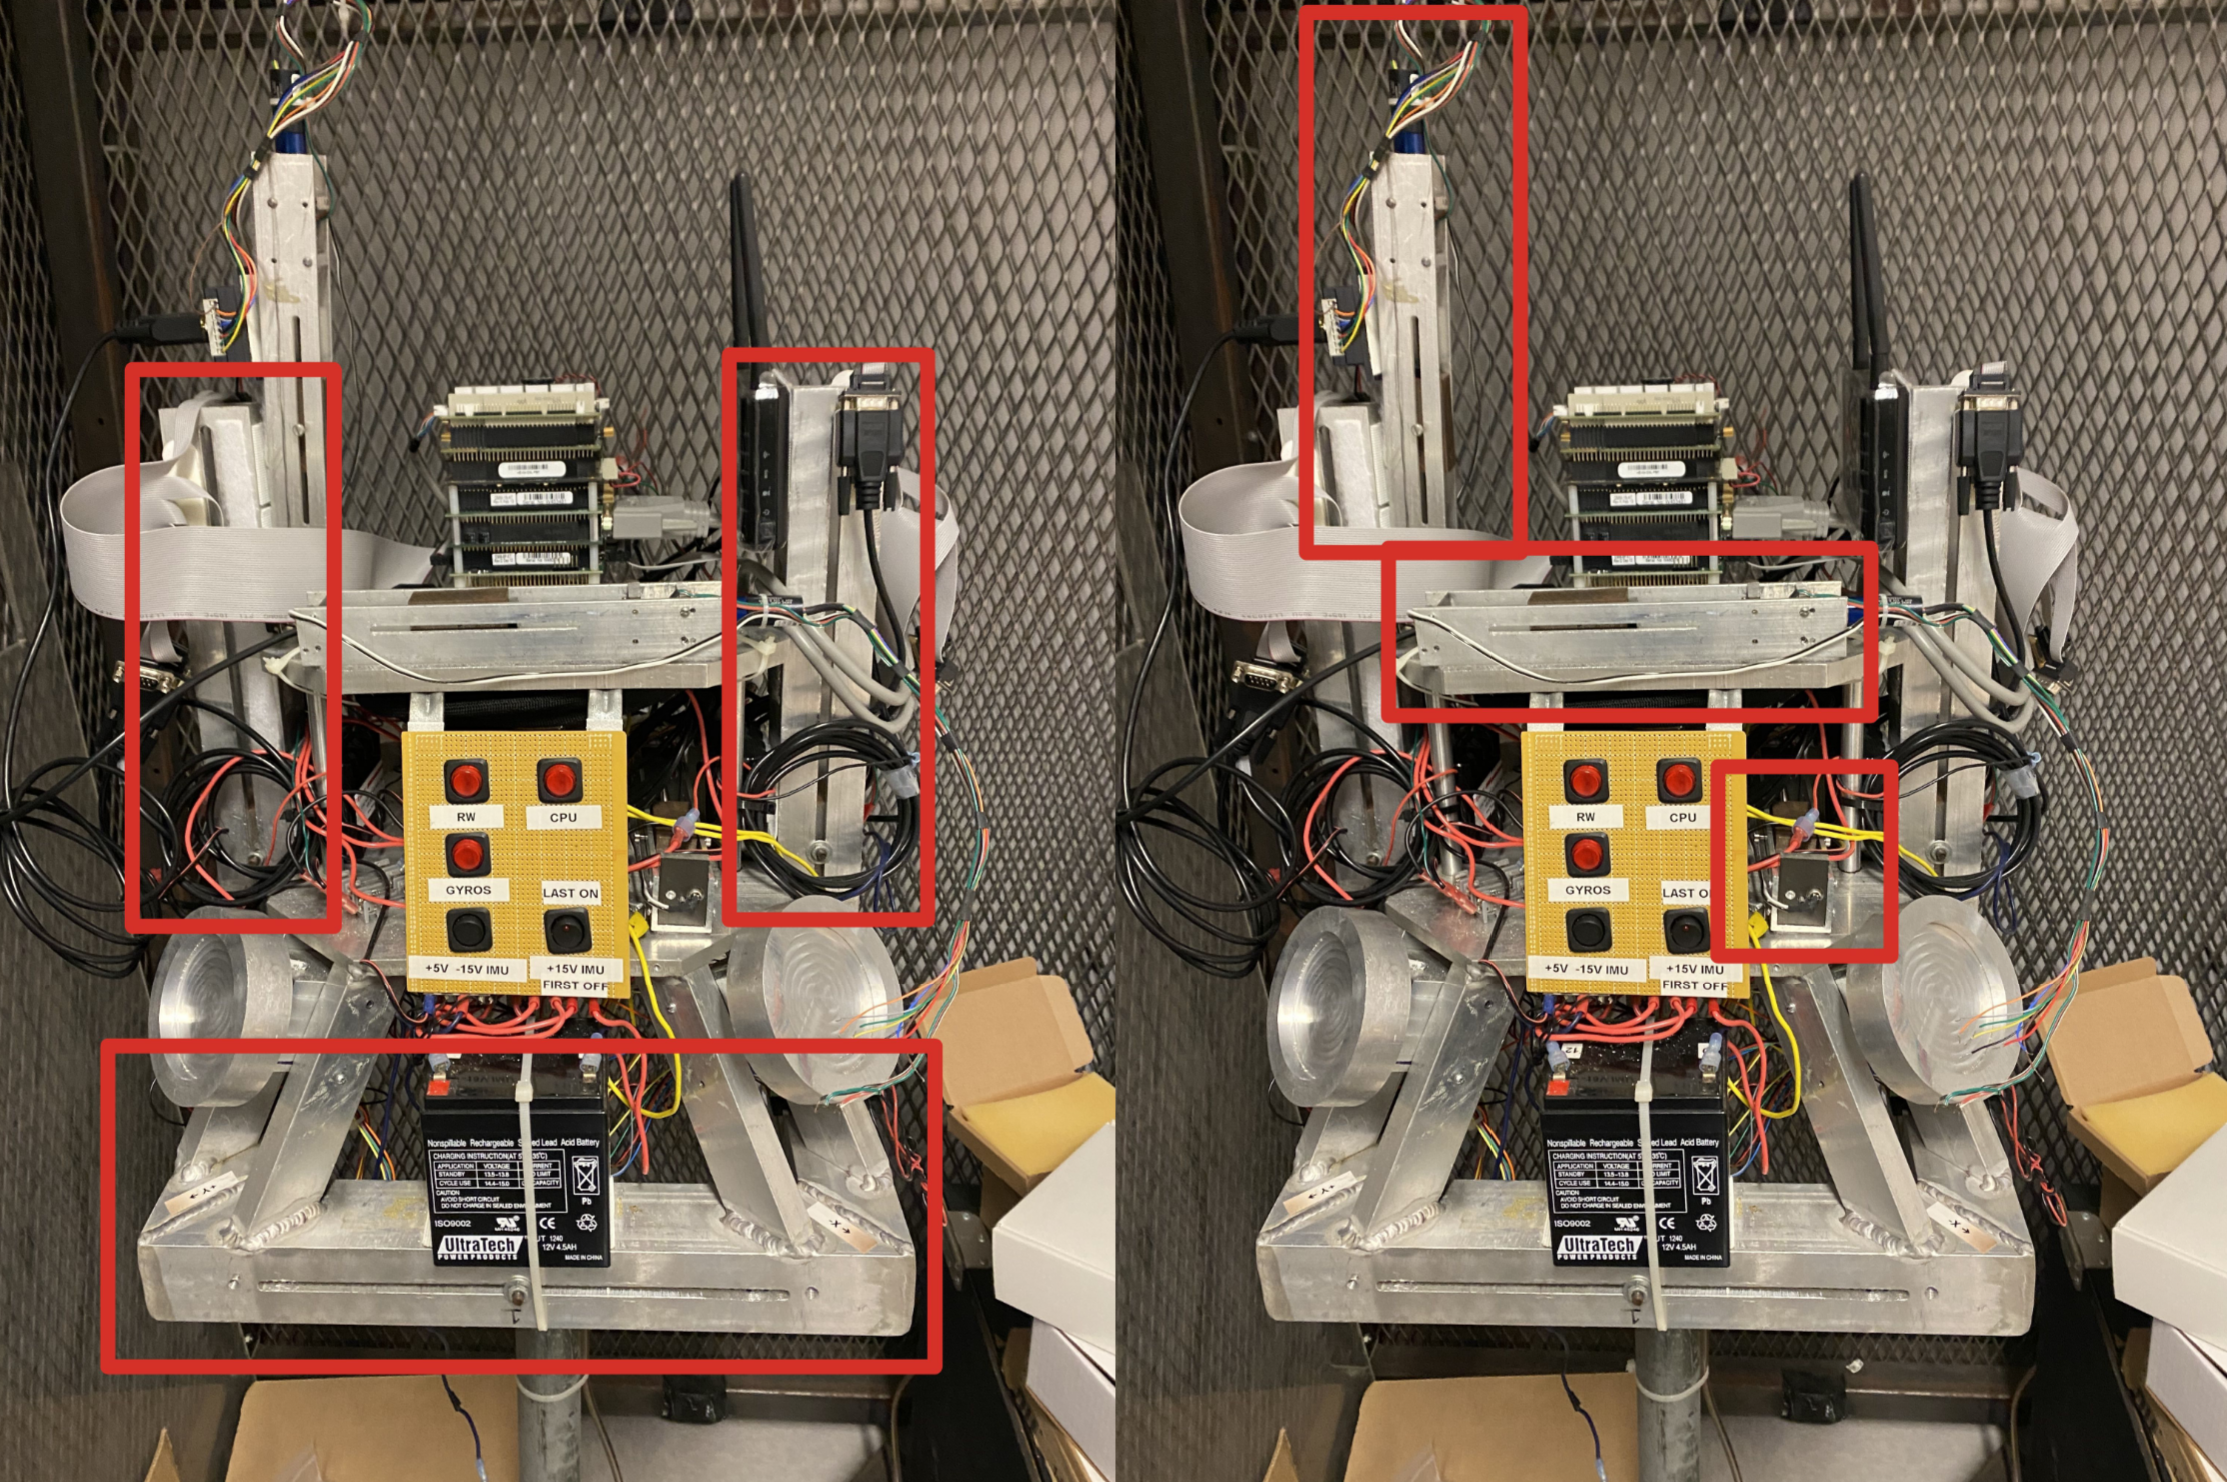
\includegraphics[width=0.90\linewidth]{figures/FMB.png}
    \caption{The coarse mass balances (left) and fine mass balances (right) on the previous iteration~\cite{gilman_automatic_2024}}
\end{figure}

The has system undergone numerous changes since 2007, some of which are detailed in \Cref{sec:previous_work}. The most relevant change is the installation of an LN-200 IMU, which has excellent noise characteristics as shown in \Cref{table:existing_testbeds}. Beginning in 2023 an effort began to completely overhaul the hardware onboard the SADS. This includes the development of a new set of reaction wheels, a new flight computer, as well as replacing the manual sliding masses with a new set controlled by linear actuators. Current reaction wheel development is documented in~\cite{nalley2025development}, which resulted in the design and integration of one complete wheel to the simulator. Work on a new flight computer remains unstarted, and development of the new mass balancing system is documented in~\cite{gilman_automatic_2024}, which resulted in the design of a new set of prototype linear actuators. 
\begin{figure}[h]\label{fig:gillman_final_work}
    \centering
    \includegraphics[width=0.70\linewidth]{figures/gillman_final_work.png}
    \caption{Linear actuator set developed in~\cite{gilman_automatic_2024}}
\end{figure}
The actuators follow the same layout as the previous iteration with six-sliding masses - two for each axis. The masses slide along a ballscrew driven by DC motors with positional feedback from rotary encoders. However when mounted on the simulator as shown in \Cref{fig:gillman_final_work}, the motors struggle to move the masses. This may be acceptable for passive balancing but is not suitable for active balancing where positions must be precisely controlled in real-time. Additionally without the flight computer, the actuators remain unproven in any real tests with a live air-bearing. 

\begin{table}[h!]
\caption{Summary of previous work on the Cal Poly Spacecraft Attitude Dynamics Simulator (SADS)}
\label{table:sads_history}
\centering
\renewcommand{\arraystretch}{1.4} % row height

\begin{tabularx}{\textwidth}{
    >{\raggedright\arraybackslash}p{4cm}   % Author/Year
    >{\raggedright\arraybackslash}p{5cm}   % Title
    >{\raggedright\arraybackslash}X}       % Notes
\hline
\textbf{Author / Year} & \textbf{Title} & \textbf{Notes} \\
\hline
Mittelsteadt, Mehiel [2007] & 
Cal Poly Spacecraft Attitude Dynamics Simulator: CP/SADS & 
First iteration of the Cal Poly SADS, purely manual balancing \\[2.0em]

Silva [2010] & 
Applied System Identification for a Four Wheel Reaction Wheel Platform & 
Introduced least squared estimation method to estimate center of mass \\[2.0em]

Dam [2014] & 
Applied Mass Properties Identification Method to the Cal Poly's Spacecraft Simulator & 
Used least squared estimation method with significantly improved measurement system \\[2.0em]

Gilman [2024] & 
Automatic Mass Balancing of a Spacecraft Attitude Dynamics Simulator with Six Sliding Masses & 
Completely replaced mass balancing hardware, only performed hardware-in-the-loop tests \\
\hline
\end{tabularx}
\end{table}

\section{Thesis Objectives}

The primary goal of this thesis is to design, integrate and test a low-cost mass balancing system that achieves similar or better balancing results than previous iterations - namely the hardware results achieved by Dam in 2014. To achieve this, work will also need to be done on the SADS' overall design \textit{still need to formalize this}
- A prototype flight computer that is compatible with Simulink Coder
- An IMU and measurement system

- provide practical insights on MBS design and implementation
- Compare the results of various balancing methods found in literature on the same platform, provide a clear comparison to simulated and real results

